\section{Numerical Experiments}
\label{sec:numerics}
We now evaluate the performance of SEGQE in numerical simulations. All results are obtained from noiseless, exact state-vector simulations.
\subsection{Transverse-Field Ising Model}
\label{sec:TFI}
To benchmark SEGQE, we approximate the ground state and ground-state energy of the transverse-field Ising (TFI) model with open boundary conditions, defined by
\begin{equation}
    \label{eq:TFI}
    H=w\sum^n_{i=1}Z_i+J\sum^{n-1}_{i=1}X_iX_{i+1},
\end{equation}
where $w$ denotes the transverse-field strength, $J$ the nearest neighbor coupling constant, and $n$ the number of spins (qubits). The gate set considered by SEGQE in this experiment includes all Pauli rotations acting on most $m=2$ qubits. The per-iteration measurement cost is therefore upper-bounded by \cref{cor:pauli-rotations}. Exploiting the structure of the Hamiltonian reduces this bound by approximately a factor of $6$ (see \cref{app:tfi}). 
\begin{figure}[htbp]
  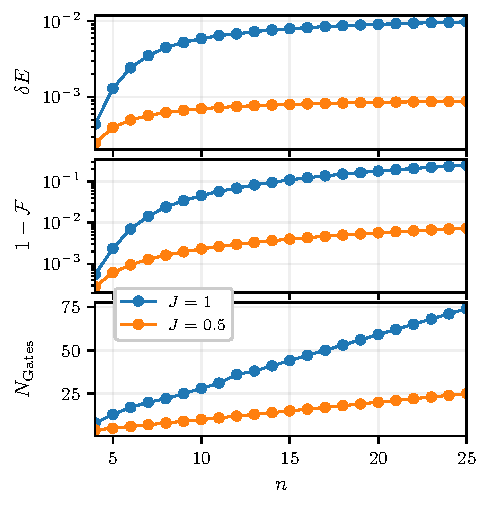
\includegraphics{figures/plot1.pdf}
  \vspace{-1em}
  \caption{Convergence properties of SEGQE applied to the open-boundary transverse-field Ising model at criticality ($J=w=1$, blue circles) and a gapped, field-dominated regime ($J=w/2$, orange circles). (Top) Relative energy error $\delta E=(E_\mathrm{exact}{-}E_\mathrm{SEGQE})/E_\mathrm{exact}$ at convergence as a function of system size $n$. (Middle) Infidelity with the exact ground state $1-\mathcal{F}$. (Bottom) Number of appended two-qubit Pauli rotations required for convergence $N_\mathrm{Gates}$. In all cases, SEGQE terminates once no candidate gate yields an energy reduction exceeding $\Delta=10^{-3}$.}
  \label{fig:2a}
\end{figure}
\Cref{fig:2a} shows the convergence properties of SEGQE applied to the open-boundary TFI model at the critical point $J=w=1$ and in a gapped, field-dominated regime $J=w/2$. In both settings, the number of SEGQE iterations, equivalently the number of appended gates $N_\mathrm{Gates}$, grows approximately linearly with system size $n$, with a slope at criticality roughly three times larger than in the gapped regime. This behavior is expected: away from criticality, correlations are short-ranged and few local rotations suffice to capture the ground state, whereas at criticality longer-range correlations emerge and must be incorporated through additional gates. 

Consistent with this picture, inspecting the circuits generated by SEGQE reveals that in the gapped regime the algorithm converges after appending only nearest-neighbor two-qubit Pauli rotations. At the critical point, SEGQE subsequently appends two additional sequences of gates acting on next-nearest and next-next-nearest neighbor qubit pairs, followed by a small number of corrective gates before terminating (see \cref{app:tfi}). This explains the larger prefactor in the linear scaling and demonstrates that SEGQE automatically adapts the circuit structure to the correlation properties of the target ground state. %In both settings, SEGQE terminates once no candidate gate yields an energy reduction exceeding the predefined threshold $\Delta = 10^{-3}$.

\Cref{fig:2a} (top) visualizes the behavior of the relative energy error $\delta E:=(E_\mathrm{exact}{-}E_\mathrm{SEGQE})/E_\mathrm{exact}$ as a function of system size. In both regimes, $\delta E$ initially increases with $n$ before leveling off, remaining below $1\%$ at criticality and below $0.1\%$ in the gapped phase across the system sizes considered. This indicates that SEGQE maintains controlled energy accuracy as the system size increases. 
Motivated by the need for approximate ground states as initial states for fault-tolerant algorithms, such as phase estimation, \cref{fig:2a} (middle) also reports the infidelity with the exact ground state, $1-\mathcal{F}=1-\left|\langle \psi_\mathrm{SEGQE}|\psi_\mathrm{exact}\rangle \right|^2$. For context, the success probability of phase estimation scales linearly with the fidelity $\mathcal{F}$, so the required repetition overhead scales as $1/\mathcal{F}$. As expected, the infidelity increases with system size, reflecting the accumulation of local imperfections. Nevertheless, this increase remains gradual over the system sizes considered and contrasts with the exponentially small overlap expected for generic random states. This suggests that SEGQE prepares structured approximations to the ground state that retain nontrivial overlap with the true ground state and may serve as suitable starting points for further processing.

\begin{figure}[htbp]
  \centering
  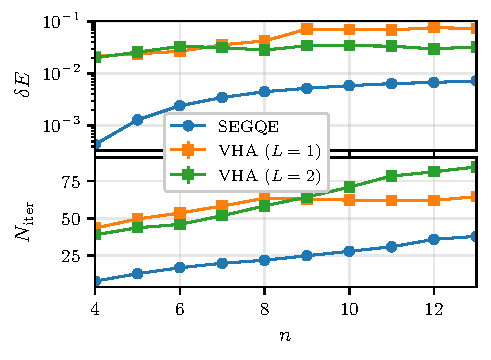
\includegraphics{figures/plot2.pdf}
  \vspace{-2em}
  \caption{Qualitative comparison between SEGQE and a variational quantum eigensolver (VQE) based on a variational Hamiltonian ansatz (VHA) applied to the open-boundary transverse-field model at the critical point $J=w=1$. (Top) Relative energy error $\delta E = (E_\mathrm{exact}{-}E)/E_\mathrm{exact}$ at convergence as a function of system size $n$. (Bottom) Number of iterations $N_\mathrm{iter}$ required for convergence. Results are shown for SEGQE (blue circles) and for VHA-VQE with one ($L=1$, orange squares) and two ($L=2$, green squares) ansatz layers. For VHA-VQE, circuit parameters are initialized randomly and results are averaged over 300 independent initializations. Error bars indicate the standard error of the mean but are smaller than the marker size. Both algorithms terminate once the energy difference between two successive iterations falls below $\Delta=10^{-3}$.
  }
  \label{fig:2b}
\end{figure}
\Cref{fig:2b} provides a qualitative comparison between SEGQE and a VQE based on a variational Hamiltonian ansatz (VHA) at criticality ($w=J=1$). We consider two VHA circuits with different expressivities, namely a single-layer ($L=1$) and a two-layer ($L=2$) ansatz. The VHA circuit is optimized using a standard gradient-based method (ADAM, with parameter-shift gradients), with all parameters initialized randomly, and results are averaged over 300 independent initializations. Across all considered systems, SEGQE converges in fewer iterations and achieves lower final energies than VHA-VQE, illustrating that SEGQE can produce competitive ground-state estimates using a greedy circuit construction. Although iteration counts are not directly comparable due to fundamentally different optimization strategies, the theoretical results of \cref{sec:guarantees} provide important context: the per-iteration sample complexity of SEGQE scales only logarithmically with system size, whereas gradient-based VHA-VQE typically requires at least $\mathcal{O}(n)$ measurements per iteration. 
\subsection{Random Local Hamiltonians}
While the TFI model provides a structured and physically motivated benchmark, it does not probe performance in unstructured settings. We therefore study SEGQE on an ensemble of random local Hamiltonians defined as
\begin{equation}
\label{eq:RLH}
\begin{aligned}  
    H=&\sum^n_{i=1}\sum_{\alpha\in\{x,y,z\}}w_i^\alpha \sigma^\alpha_i\\+&\sum^n_{i=1}\sum_{\alpha,\beta\in\{x,y,z\}}J^{\alpha \beta}_i\sigma_i^\alpha\sigma_{(i+1)\mod n}^\beta,
\end{aligned} 
\end{equation}
where the coefficients $w_{i}^\alpha$ and $J_i^{\alpha \beta}$ are drawn independently from $\mathcal{N}(0,1)$. Here, $\sigma^\alpha_i$ denotes the Pauli operator $\sigma^\alpha\in \{X,Y,Z\}$ acting on qubit $i$, and periodic boundary conditions are imposed.
\begin{figure}
  \centering
  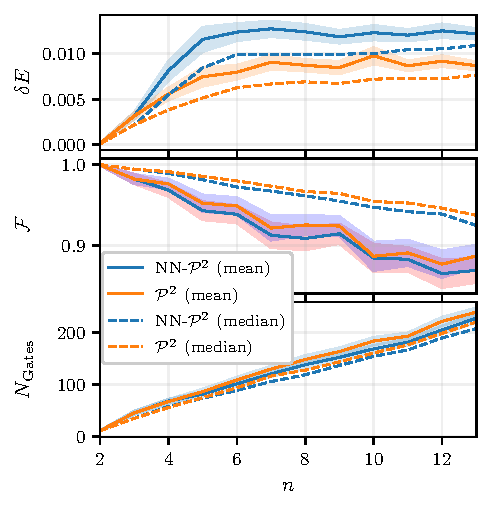
\includegraphics{figures/plot3.pdf}
  \vspace{-1em}
  \caption{Convergence properties of SEGQE applied to 500 instances of the random local Hamiltonians defined in \cref{eq:RLH}. (Top) Relative energy error $\delta E=(E_\mathrm{exact}{-}E_\mathrm{SEGQE})/E_\mathrm{exact}$ at convergence as a function of system size $n$. (Middle) Ground-state fidelity $\mathcal{F}$. (Bottom) Number of appended two-qubit gates required for convergence $N_\mathrm{Gates}$. Results are shown for SEGQE using all two-qubit Pauli rotations ($\mathcal{P}^2$, orange) and for the restriction to nearest-neighbor two-qubit Pauli rotations (NN-$\mathcal{P}^2$, blue). Solid lines indicate the mean over all considered instances, dashed lines the median. Shaded regions indicate the two-sigma confidence interval of the mean. In all cases, SEGQE terminates once no candidate gate yields a maximal energy reduction exceeding $\Delta=10^{-3}$.
  }
  \label{fig:a}
\end{figure}

\Cref{fig:a} shows the convergence properties of SEGQE applied to the ensemble of local Hamiltonians defined in \cref{eq:RLH}, considering two different gate sets: all two-qubit Pauli rotations and their restriction to nearest-neighbors. In both cases, the number of appended gates required for convergence grows approximately linearly with system size $n$, consistent with the behavior observed for the TFI model. Across the system sizes considered, the relative energy error depends only weakly on $n$ and appears to saturate at the percent level, while the ground-state fidelity decreases approximately linearly. Restricting SEGQE to nearest-neighbor gates leads to systematically worse energy accuracy and ground-state fidelity, indicating that longer-range two-qubit rotations are important to accurately capture the ground states of these unstructured Hamiltonians. 

The weak system-size dependence of the final energy error can be understood from the local and random nature of the considered Hamiltonians. In one-dimensional chains with random couplings, ground-state correlations typically decay rapidly with distance, yielding a finite correlation length on average. Importantly, this does not imply that correlations are strictly limited to nearest neighbors. Rather, accurately capturing the ground state generally requires incorporating correlations over a small but finite range. This is consistent with our observation that allowing a limited number of longer-range two-qubit rotations significantly improves energy accuracy, while further extensions of the interaction range yield diminishing returns, explaining the observed mild growth and apparent saturation of the energy error with increasing system size.

To further investigate the dependence of SEGQE on the choice of gate set, \cref{fig:b} plots the relative energy error $\delta E$ as a function of the number of appended gates $N_\mathrm{Gates}$ at fixed system size ($n=5$) for four distinct gate sets: 2-qubit Pauli rotations ($\mathcal{P}^2$), arbitrary 2-qubit gates ($\mathrm{SU}(4)$), and their restrictions to nearest-neighbor qubits, denoted NN-$\mathcal{P}^2$ and NN-$\mathrm{SU}(4)$. 
\begin{figure}[htbp]
  \centering
  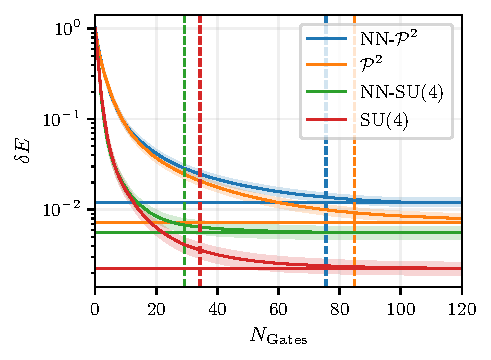
\includegraphics{figures/plot4.pdf}
  \caption{Dependence of SEGQE convergence on gate-set for random local Hamiltonians at fixed system size $n=5$. Shown is the relative energy error $\delta E=(E_\mathrm{exact}{-}E_\mathrm{SEGQE})/E_\mathrm{exact}$ as a function of the number of appended gates $N_\mathrm{Gates}$ for four gate sets: nearest-neighbor two-qubit rotations (NN-$\mathcal{P}^2$, blue), arbitrary-distance two-qubit Pauli rotations ($\mathcal{P}^2$, orange), nearest-neighbor arbitrary two-qubit unitaries (NN-$\mathrm{SU}(4)$, green), and arbitrary-distance two-qubit unitaries ($\mathrm{SU}(4)$, red). Solid lines indicate the mean over 100 independent random Hamiltonian instances, and shaded regions indicate the one-sigma confidence interval of the mean. Horizontal lines show the average final energy error at convergence for each gate set, while vertical dashed lines indicate the corresponding average number of appended gates at convergence. SEGQE terminates once no candidate gate yields a maximal energy reduction exceeding $\Delta=10^{-3}$. 
  }
  \label{fig:b}
\end{figure}
Two distinct effects can be observed. First, for a fixed gate geometry, allowing arbitrary two-qubit unitaries leads to lower final energies and faster convergence, reflecting the increased local expressivity when considering all of $\mathrm{SU}(4)$. Second, restricting the gate set to nearest neighbors results in earlier saturation at higher energy, indicating that geometric restrictions limit the correlations that can be captured. The plot further shows that while nearest-neighbor variants converge more rapidly, this behavior reflects premature convergence rather than more efficient optimization. Overall, these results indicate that both increased local gate expressivity and longer-range interactions improve the achievable energy accuracy, highlighting that SEGQE should exploit richer gate sets when available. Finally, we note that in the simulations shown here, the classical optimization over $\mathrm{SU}(4)$ required fewer than $T=2\times 10^4$ function evaluations for each appended gate. Although this may appear costly, the logarithmic dependence of the SEGQE sample complexity on the size of the gate set (see \cref{sec:guarantees}) ensures that this overhead remains moderate. For example, fixing the confidence parameter to $\delta=0.01$, increasing the optimization budget from $T=100$ to $T=2\times 10^4$ increases the required number of measurements by a factor of less than $1.5$ for the $5$-qubit system considered in \cref{fig:b}. Assuming that the number of required function evaluations does not increase with system size, this relative overhead becomes even less pronounced for larger systems.

